\documentclass{article} % For LaTeX2e
\usepackage{final_project,times,graphicx}
%\documentstyle[nips12submit_09,times,art10]{article} % For LaTeX 2.09


\title{Predicting the Impact of Research Papers in the Covid-19 Open Research Dataset}



\author{
Tyler Ashoff \\
Department of Interdisciplinary Data Science\\
Duke University\\
Durham, NC 27708 \\
\texttt{tyler.ashoff@duke.edu} \\
\\
\textbf{Jennifer Wilson} \\
Department of Statistical Science\\
Duke University\\
Durham, NC 27708 \\
\texttt{jennifer.wilson994@duke.edu} \\
}

\newcommand{\fix}{\marginpar{FIX}}
\newcommand{\new}{\marginpar{NEW}}

\nipsfinalcopy

\begin{document}


\maketitle



\begin{abstract}
The volume of research papers and articles relating to Coronaviruses combined with the rapid increase at which new information is being published makes it nearly impossible for those relying on this research to keep up [1]. We propose the use of citation count prediction [2] to identify impactful articles which may have been overlooked.
\end{abstract}

\section{Introduction}

As the world community became engulfed in the Covid-19 pandemic in early 2020, the scientific community sprang into action. The rate at which new results and research are still being published at an alarming rate. In an effort to help identify potentially influential research, we turn to citation count prediction.

Citation count prediction is one of a number of methods for predicting the importance and popularity of a paper [2]. While numerous modeling methods have already been produced to predict this, we look at citation count prediction specifically as it relates to the Covid-19 Open Research Dataset (COORD) [1]. This dataset compiled by the Whitehouse and leading researchers provides information on over 57,000 articles, including the full text. This dataset provides some unique challenges related to the steep rise in articles recently published resulting in a dataset that is highly skewed. Additionally, the does not include information heavily relied on for citation count prediction such as the h-index [3]. Therefore we focus on extracting data from the documents and abstracts themselves in an attempt to predict citation count. Numerous different modeling techniques were attempted, including neural nets, zero-inflated poisson regression, hierarchical modeling and gradient boosting. Many of these models had little to no significance. 

\section{Data Wrangling}
\label{headings}

First level headings are lower case (except for first word and proper nouns),


\subsection{Headings: second level}

Second level headings are lower case (except for first word and proper nouns),


\section{Methods}
\label{others}

These instructions apply to everyone, regardless of the formatter being used.

\subsection{Transformations}
Transformations of the response and covariates proved to have significant impact on model performance. Most gains in improving results came from transformations as opposed to tuning parameters.

\subsubsection{Response}
A significant number of articles in this dataset have no citations. While some of this is simply due to the fact that they have not been published long enough for others to have cited them yet, this phenomenon is still present when restricting to articles published in previous years. Additionally, there are some articles that receive a significantly large number of citations. We opt to use a $log(x+1)$ transformation on the response which allows us to normalize the non zero counts and futher separate articles with citations from those without. While not among the final models we present, we did attempt a zero inflated poisson model without the transformation to try and deal with the high mass at zero. This model had poor results.


\begin{figure}[h]
\begin{center}
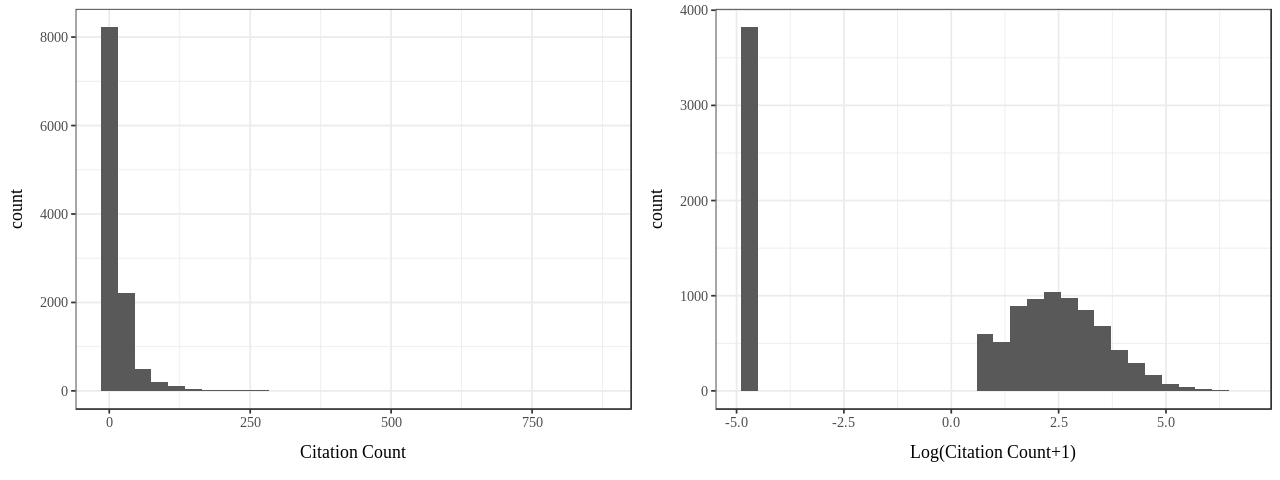
\includegraphics[scale=0.5]{../probML_project/Figures/citation_hist.png} 
\end{center}
\caption{Transformation of Citation Count}
\end{figure}


\subsubsection{Covariates}
Many of the covariates from the embedding task were not linearly related to the citation counts. Most often this appeared as a high citation count and lots of density near a value of 0 with low citation counts in the positive and negative limits with low density. We use a $log(x^2)$ transformation of these covariates. While somewhat convoluted and uninterpretable, this transformation does a good job at spreading out the distribution of the data and linearizing the relationship. Additionally, any count related covariates were given a log transformation.




\subsection{Figures}

All artwork must be neat, clean, and legible. Lines should be dark
enough for purposes of reproduction; art work should not be
hand-drawn. The figure number and caption always appear after the
figure. Place one line space before the figure caption, and one line
space after the figure. The figure caption is lower case (except for
first word and proper nouns); figures are numbered consecutively.

Make sure the figure caption does not get separated from the figure.
Leave sufficient space to avoid splitting the figure and figure caption.


\begin{figure}[h]
\begin{center}
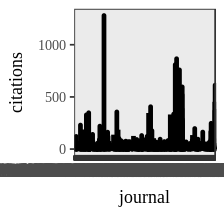
\includegraphics[scale=0.5]{../probML_project/Figures/test1.png} 
\end{center}
\caption{Sample ggplot}
\end{figure}


\subsection{Tables}

All tables must be centered, neat, clean and legible. Do not use hand-drawn
tables. The table number and title always appear before the table. See
Table~\ref{sample-table}.

Place one line space before the table title, one line space after the table
title, and one line space after the table. The table title must be lower case
(except for first word and proper nouns); tables are numbered consecutively.


% latex table generated in R 3.5.0 by xtable 1.8-2 package
% Sat May  2 12:28:59 2020
\begin{table}[ht]
\centering
\caption{Xtable Example} 
\begin{tabular}{rl}
  \hline
 & Features \\ 
  \hline
1 & Journal name \\ 
  2 & Publication year \\ 
  3 & Average abstract distance \\ 
  4 & Six month average abstract distance \\ 
  5 & Count of close abstracts \\ 
  6 & Average body distance \\ 
  7 & Six month average body distance \\ 
  8 & Count of close bodies \\ 
   \hline
\end{tabular}
\end{table}





\subsubsection*{Acknowledgments}

Use unnumbered third level headings for the acknowledgments. All
acknowledgments go at the end of the paper.

\subsubsection*{References}

References follow the acknowledgments. Use unnumbered 

\small{
[1] Allen Institute For AI. “COVID-19 Open Research Dataset Challenge (CORD-19).” Kaggle, CDC, 25 Apr. 2020, www.kaggle.com/allen-institute-for-ai/CORD-19-research-challenge.

[2] Yan, Rui \& Tang, Jie \& Liu, Xiaobing \& Shan, Dongdong \& Li, Xiaoming. (2011). Citation count prediction: Learning to estimate future citations for literature. {\itInternational Conference on  Information and Knowledge Management, Proceedings} 1247-1252. 10.1145/2063576.2063757. 

[3] J. Hirsch. An index to quantify an individual’s scientific
research output. Proceedings of the National Academy of
Sciences of the United States of America, 102(46):16569,
2005.
}


\end{document}
